\ifpdf
    \graphicspath{{9_backmatter/figures/PNG/}{9_backmatter/figures/PDF/}{9_backmatter/figures/}}
\fi


% \chapter{Disabilities Classification}
% \label{cha:appendixA}
% 
% Researchers have developed and improved several techniques to model users for 
% the past 20 years~\citep{petrelli_user_centered_1999} \citep{fink_adaptable_1997}. 
% Modelling users needs to gather knowledge about their capabilities, drawbacks and 
% limitations. During these first decades there was not any official and medical-based 
% study to consult about user capabilities. Nevertheless, in 2001 this situation 
% changed. Under the \ac{who} coordination the World Health Assembly published the
% \ac{icf} document. \ac{icf} is a classification of human functioning and disability. 
% It classifies every function state associated with health (e.g., diseases, 
% disruptions, injuries and traumas). Its purpose is to identify the low-level 
% capabilities relevant to product design in several domains. As was written by 
% experts in the area, the \ac{icf} document is a reference for identifying several 
% user capabilities in any interaction process. Its goals are the following:
% 
% \begin{itemize}
%   \item To provide a scientific basis for understanding and studying health and
%   health-related states, outcomes and determinants.
%   \item To establish a common language for describing health and health-related 
%   states in order to improve communication between different users, such as health 
%   care workers, researchers, policy-makers and the public, including people with 
%   disabilities.
%   \item To permit comparison of data across countries, health care disciplines,
%   services and time.
%   \item To provide a systematic coding scheme for health information systems.
% \end{itemize}
% 
% It is organized into two main groups: Part 1 deals with \textit{Functioning and
% Disability}; Part 2 covers \textit{Contextual Factors}. From the first group the 
% following categories are highlighted:
% 
% \begin{itemize}
%   \item Body functions.
%   \item Body structures.
%   \item Activities and participation.
%   \item Environmental factors.
% \end{itemize}
% 
% The second group gathers a list of \textit{Environmental Factors} which have an 
% impact on all components of functioning and disability.
% 
% \ac{icf} considers 8 main components in the context of health:
% 
% \begin{description}
%   \item[\Defi{Body functions}] \hfill \\
%     \begin{mdframed}[hidealllines=true,backgroundcolor=gray!20]
%     \textit{``Body functions are the physiological functions of body systems (including
%     psychological functions)''.}
%     \end{mdframed}
% % 
%   \item[\Defi{Body structures}] \hfill \\
%     \begin{mdframed}[hidealllines=true,backgroundcolor=gray!20]
%     \textit{``Body structures are anatomical parts of the body such as organs, 
%     limbs and their components''.}
%     \end{mdframed}
%     
%   \item[\Defi{Impairments}] \hfill \\
%     \begin{mdframed}[hidealllines=true,backgroundcolor=gray!20]
%     \textit{``Impairments are problems in body function or structure such as a 
%     significant deviation or loss''.}
%     \end{mdframed}
% 
%   \item[\Defi{Activity}] \hfill \\
%     \begin{mdframed}[hidealllines=true,backgroundcolor=gray!20]
%     \textit{``Activity is the execution of a task or action by an individual''.}
%     \end{mdframed}
% 
%   \item[\Defi{Participation}] \hfill \\
%     \begin{mdframed}[hidealllines=true,backgroundcolor=gray!20]
%     \textit{``Participation is involvement in a life situation''.}
%     \end{mdframed}
% 
%   \item[\Defi{Activity limitations}] \hfill \\
%     \begin{mdframed}[hidealllines=true,backgroundcolor=gray!20]
%     \textit{``Activity limitations are difficulties an individual may have in 
%     executing activities''.}
%     \end{mdframed} 
%     
%   \item[\Defi{Participation restrictions}] \hfill \\
%     \begin{mdframed}[hidealllines=true,backgroundcolor=gray!20]
%     \textit{``Participation restrictions are problems an individual may experience 
%     in involvement in life situations''.}
%     \end{mdframed}
% 
%   \item[\Defi{Environmental factors}] \hfill \\
%     \begin{mdframed}[hidealllines=true,backgroundcolor=gray!20]
%     \textit{``Environmental factors make up the physical, social and attitudinal
%     environment in which people live and conduct their lives''.}
%     \end{mdframed} 
% \end{description}
% 
% 
% 
% Figure~\ref{fig:icf_interaction} illustrates how these components interact.
% 
% \begin{figure}
% \centering
% 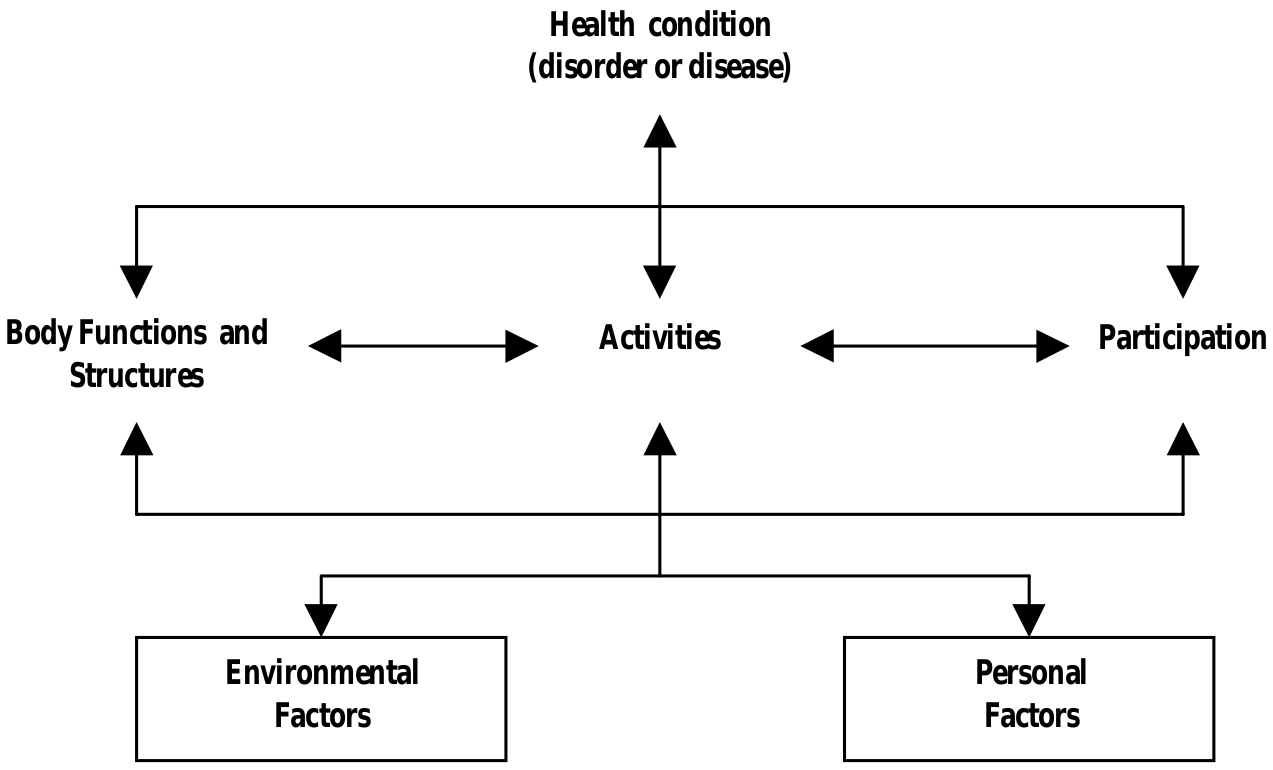
\includegraphics[width=0.75\textwidth]{icf_interaction.png}
% \caption{Interactions between the components of~\ac{icf}.}
% \label{fig:icf_interaction}
% \end{figure}







Due to the nature of user capabilities, in this dissertation we take the very 
first category as the official reference to model users as it is directly 
related to \ac{hci}. This category encompasses the following functions:

\begin{itemize}
  \item Mental functions.
  \item Sensory functions and pain.
  \item Voice and speech functions.
  \item Neuromusculoskeletal and movement-related functions.
\end{itemize}


\citeauthor{persad_cognitive_2007} also reviewed functional classifications 
and experimental studies to identify the most relevant low-level skills for 
designing products within the cognitive, motor and sensory domain:

\paragraph*{Sensory capabilities}
\subparagraph*{Visual capabilities} Several sensory capabilities are known to 
deteriorate with ageing~\citep{persad_exploring_2006}. Thus, 
\citeauthor{persad_exploring_2006} stated that the following functions seem to 
account for most of visual disability:

\begin{itemize}
  \item Visual acuity.
  \item Contrast sensitivity.
  \item Colour perception.
  \item Useful field of view.
  \item Stereopsis.
\end{itemize}


\subparagraph*{Hearing capabilities} Loss of hearing capabilities may directly 
affect the speech interaction with the device. The main low-level hearing 
functions to guarantee the interaction are the following:

\begin{itemize}
  \item Pure tone detection thresholds.
  \item Speech detection and recognition discrimination thresholds.
  \item Sound localization.
\end{itemize}

% \subparagraph*{Environmental effects}
% The level of illumination, noise, weather, etc. are several environment features 
% which might affect user capabilities.

\paragraph*{Cognitive capabilities}
The product's user interface must be usable and accessible enough to guarantee 
that users easily understand the interaction. The following capabilities are 
related to the human cognitive domain:

\begin{itemize}
 \item Working memory performance.
 \item Long term memory.
 \item Mental models, planning and problem solving.
 \item Language and communication capabilities.
\end{itemize}

\paragraph*{Motor capabilities}
\subparagraph*{Upper limb capabilities}
There are many conditions that affect manipulating a product (e.g., arthritis, 
stroke, multiple sclerosis, head injury, cerebral palsy and missing or damaged 
limbs). These problems directly reduce grasp forces, range of motion and fatigue 
thresholds~\cite{persad_characterising_2007}.

The following areas are highlighted within motor capabilities:
\begin{itemize}
  \item Reach ranges for each arm.
  \item Grasping, dexterity and force exertion.
  \item Two handed actions and coordination.
\end{itemize}

\subparagraph*{Gross body movement capabilities}
Usually products require certain user mobility degree. 
\\
Besides, \citeauthor{persad_characterising_2007} provide six general categories 
for product features and their interface classification. For this classification 
their toaster case study is considered (see Table~\ref{tbl:persad_product_interface}).

\begin{table}
  \caption{Product interface classification by~\citet{persad_characterising_2007}.}
  \label{tbl:persad_product_interface}
\footnotesize
\centering
    \begin{tabular}{l l}
    \hline
    \textbf{Feature type} & \textbf{Examples} \\
    \hline
    Product chassis & Handles, gripping surface \\
    Displays and indicators & Visual and auditory displays \\
    Controls and control groups & Discrete controls (Button, Switch) and continuous\\
    & controls (Slider, Knob, thumb, wheel, dial, joystick). \\
    & Control groups \textit{Keypad} \\
    Material/media input and output & Slots (toaster slots), powered and un-powered\\
    & bays and trays, doors, lids and covers\\
    Connectors for energy and data & Power and data connectors \\
    Software interfaces & Navigation menus and GUI objects \\
    \hline
  \end{tabular}
\end{table}